\chapter{相关技术的研究使用}
本章主要介绍了一些已有的CPU/GPU异构计算优化方法和编译原理中一些调整代码序列的方法,
通过对已有的优化方法进行总结比较,提出本文一种基于代码移动来迁移、合并核函数的数据交换
操作的优化方法。

\section{GPU编程优化方法}
GPU的物理结构更加适合大数据、高并发的复杂计算,任何优化GPU编程的方法都是基于GPU物理
特性充分发挥GPU计算性能来实现的。本节将介绍、对比一些业界主流的GPU编程优化方法以及
每种方法的使用场景。

\subsection{向量化}
\begin{figure}
\centering
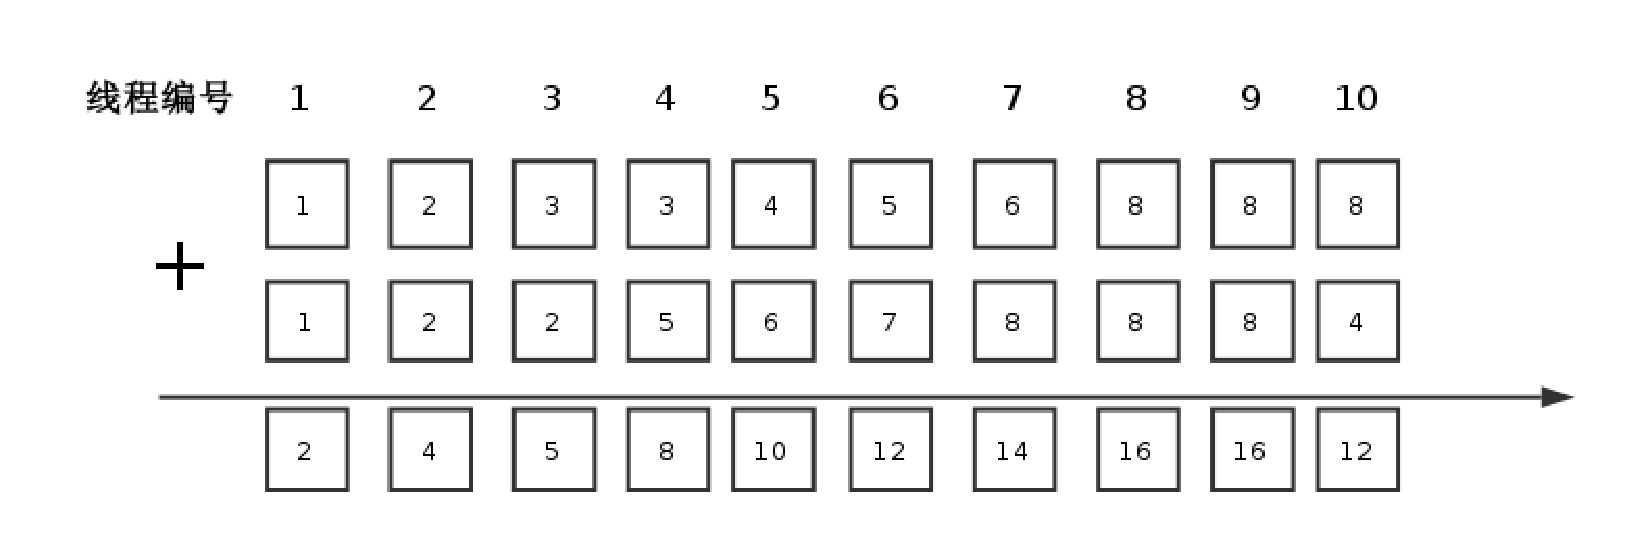
\includegraphics[width=0.9\linewidth]{figure3.eps}
\caption{向量化}\label{figure3}
\end{figure}
程序员可以在编写代码之前手动分析GPU应用程序中数据特点,再根据GPU结构特性去确定如何组织、存储、访问
数据以及确定程序逻辑可以达到优化程序的目的。向量计算是图像算法中经常使用的计算方法,我们可以使用
数组很好地表示一维向量进行计算。但是在向量乘法、加法等计算操作中,向量中每一个维度的操作基本都是相同
而且相互不干扰的,具有很高的并行性。核函数中使用数组表示一维向量时,在向量计算中仅仅使用了
单个线程循环迭代处理向量中每个维度的计算,没有利用到向量的计算并行性和GPU的多核特点,效率较低。
主流GPU编程语言CUDA和OpenCL都提供了数据向量化方法,用专有的数据结构去表示向量。如图~\ref{figure3}所示,向量化后的计算,
每一个维度的的操作都会分配到不同核心上的
线程执行,不再是整个向量维度的计算都在一个线程上。
向量化的数据结构在GPU中计算时可以充分利用GPU多核特性
,每一个维度的计算都放在了不同核心上的线程,可以加速向量计算。

\subsection{优化GPU内存使用}
第一章简单描述了GPU内存结构,较为复杂,由常量内存、
纹理内存、共享内存和全局DRAM等组成。不同种类的存储器特点和适用场景差别很大,表~\ref{table1}
简单列出了不同GPU储存器的一些特点,GPU程序员必须要清楚地了解
GPU的内存特点再根据使用场景具体选择。
编写代码时,如何设计数据在GPU内存中的存储方式也是一种很重要的优化GPU程序的方法。
寄存器是GPU计算单元访问延迟最低的存储器,GPU程序运行时会自动将一些中间数据存储到
寄存器上加速下次读取。但是GPU会将一些线程私有变量存到线程的寄存器上,程序员定义了过多的线程私有变量
会导致程序运行时一些GPU线程内寄存器不足,换而使用显卡中的局部内存,增加了访问延迟。
我们可以把GPU运行时不发生变化的数据存储到GPU常量内存中,单个线程对
常量内存中数据的访问会使GPU将该数据广播到同一线程束中的其他线程,由此可以减少整个程序对常量内存
的读取次数。
\begin{table}[b]
  \centering
  \caption{GPU内存特性}
  \begin{tabular}{llll}
    \hline
    存储器     & 位置      & 访问权限 & 变量生存周期    \\
    \hline
    寄存器     & GPU片上   & GPU可读/写  & 与线程相同    \\
    局部存储器 & 板载显卡  & GPU可读/写  & 与线程相同    \\
    共享内存   & GPU片上   & GPU可读/写  & 与线程块相同   \\
    常量内存   & 板载显卡  & CPU/GPU可读/写  &  与程序相同     \\
    纹理内存   & 板载显卡  & CPU/GPU可读/写  &  与程序相同         \\
    全局内存   & 板载显卡  & CPU/GPU可读/写  &  与程序相同  \\

    \hline
  \end{tabular}
  \label{table1}
\end{table}
共享内存是GPU片上线程块内所有线程可以读写的共享存储空间,是线程块内线程数据交互延迟最低的通信方式。
当程序中一些数据是线程块内所有线程共享的,我们可以使用共享内存代替全局内存,降低线程之间相互通信的延迟。
纹理内存也是GPU中只读内存,被设计用来存储空间局部性比较高的数据。由于GPU结构中没有
cache来缓存时间局部性的数据,如何利用好数据的空间局部性就是一个很重要的优化方法。特别是在图形计算中
,每个像素点的在空间上的联系非常紧密,空间复杂度很高,使用纹理内存的读取特性可以很容易读取空间上联系
紧密的数据,加速内存访问速度。
%CUDA和OpenCL都提供了纹理内存的使用接口,程序员可以根据具体应用数据访问的空间局部性决定是否使用纹理内存。
综合本小节的描述可以看出,GPU中不同内存的性质差别很大,根据具体场景选择
合适的存储器将会很大程度上优化GPU程序。

\subsection{嵌套循环展开}
\begin{figure}[!h]
\centering
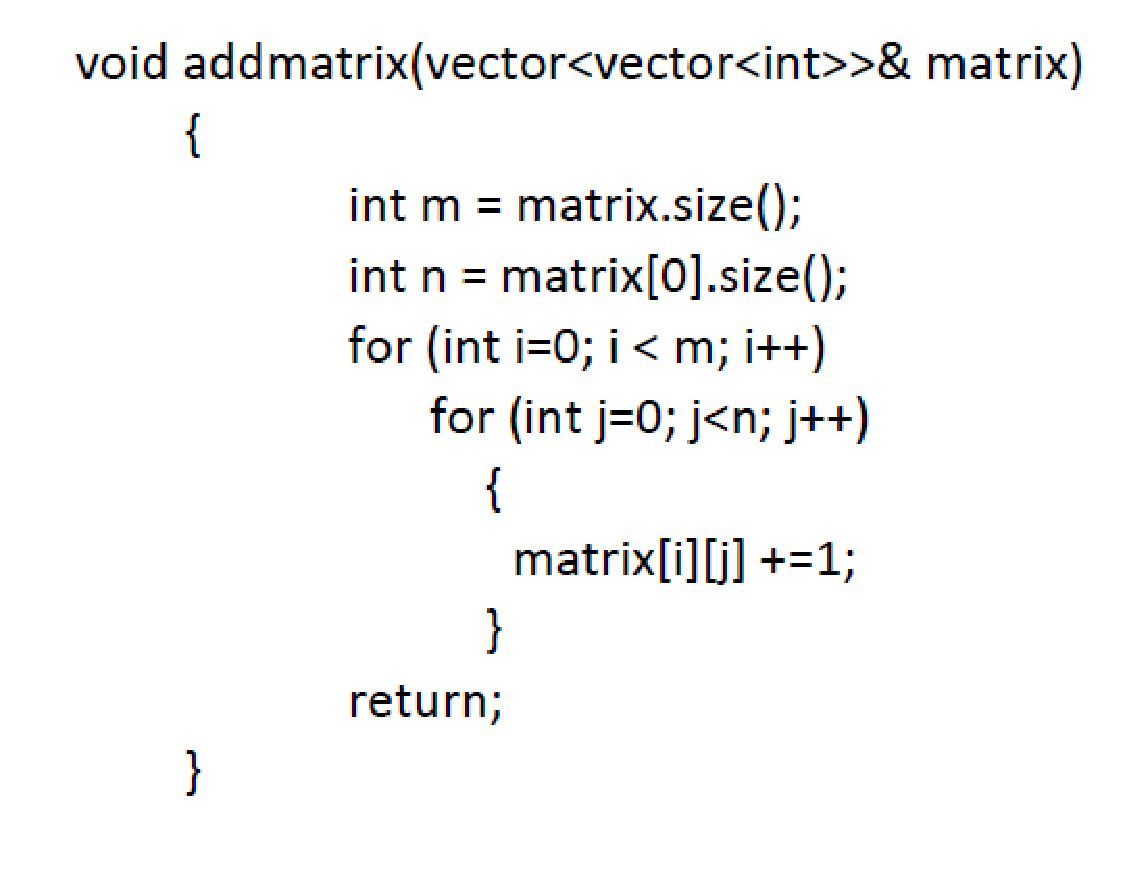
\includegraphics[width=0.8\linewidth]{figure4.eps}
\caption{嵌套循环}\label{figure4}
\end{figure}

\begin{figure}[!h]
\centering
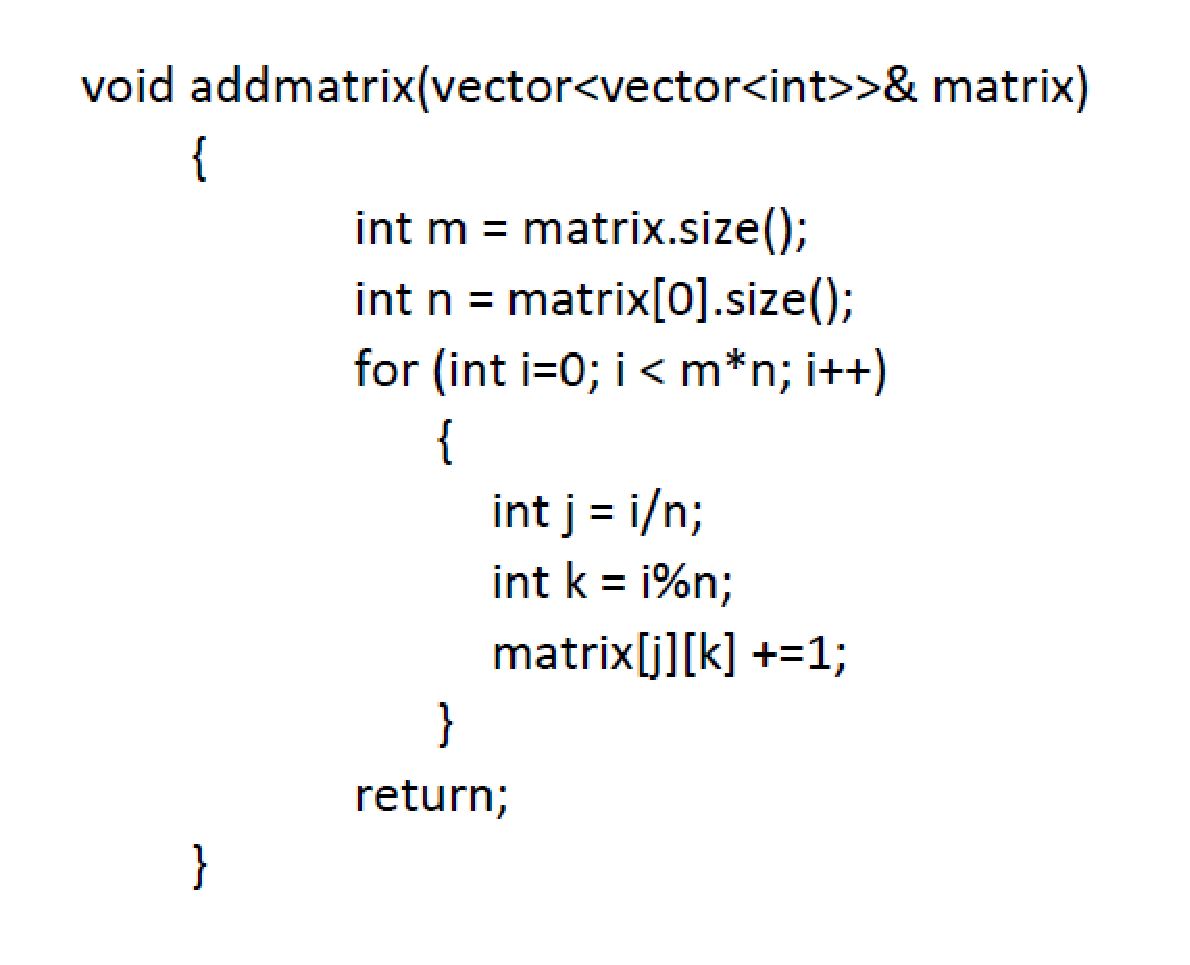
\includegraphics[width=0.8\linewidth]{figure5.eps}
\caption{嵌套循环展开}\label{figure5}
\end{figure}
GPU之所以能够快速处理大数据并行计算是因为其拥有很多个计算核心,可以同时运行多个线程。GPU程序中的核函数都是
一些计算量很大的循环结构,循环结构中每一次迭代都是独立的,这样GPU就可以启动很多个线程去运行循环结构中的每一次
迭代计算。由此可见,循环结构的迭代次数越多,加速效果越明显。但是GPU程序中循环不都是简单的单层循环,更常见的是
逻辑比较复杂的多层嵌套循环。
在核函数里的多层嵌套循环结构中,只有最里层的循环结构是同时在不同线程上计算的。这样的计算方式使得
嵌套循环结构没有完全利用GPU的多核优势,闲置了很多计算资源。
嵌套循环展开是指预处理GPU程序时把一些核函数中的二层或者多层嵌套循环展开、合并成单个循环。
如图~\ref{figure4}、~\ref{figure5}所示两段代码都是实现了一个矩阵所有元素加1的简单操作。显然两段代码的时间复杂
都是相同的,嵌套展开后的代码段还增加了计算举证行、列索引的操作。如果在普通CPU上执行的话,显然图~\ref{figure4}
中的代码段执行的会更快,因为CPU是没有足够的计算单元来开启多个线程并行计算该循环的。但是GPU的多核特性正是针对
处理并行程度高的计算的,图~\ref{figure5}把图~\ref{figure4}中的嵌套循环合并成一个迭代比较大的单个循环,这样允许
GPU开启更多的线程去计算该核函数,得到更好的优化效果。这里只拿矩阵自加作为例子介绍嵌套循环展开,当计算比较复杂,
每一次迭代的计算量都比较大时,嵌套循环展开对GPU核函数的优化将是十分明显的。


\subsection{线程配置}
本小节以CUDA平台为例简单描述GPU编程中的线程配置。CUDA的线程设计以网格(Grid)、线程块(Block)和线程(Thread)组成,
具体结构如图~\ref{figure6}所示。GPU上所有的计算单元被划分为两到三个网格,每个网格包含一定数量的线程块,目前
最多为65535个线程块,每个线程块再由一定数量的线程组成,目前主流显卡线程块最多可以包含1024个线程。如何配置好
如此多的线程对GPU程序员将是一个很大的挑战,也是优化GPU程序一个很重要的维度。同一线程块内的线程具有相同的指
令地址,不但能够并发执行,而且可以通过GPU片上共享内存和栅栏实现块内快速通信。这样,程序员在设计CUDA程序时需要
优先把相互通信量较大、较为频繁或者需要同步的线程分配到同一线程块内,利用共享内存降低线程通信延迟,同时把不需
要通信的线程分配到不同线程块内,使其并行粒度更高。CUDA架构通过块间粗粒度并行,块内细粒度并行两种方式来组织线程。
多个计算单元加上一些寄存器和共享存储器组成一个多元处理器。每个线程块最终都是交给一个多元处理器执行的。
\begin{figure}
\centering
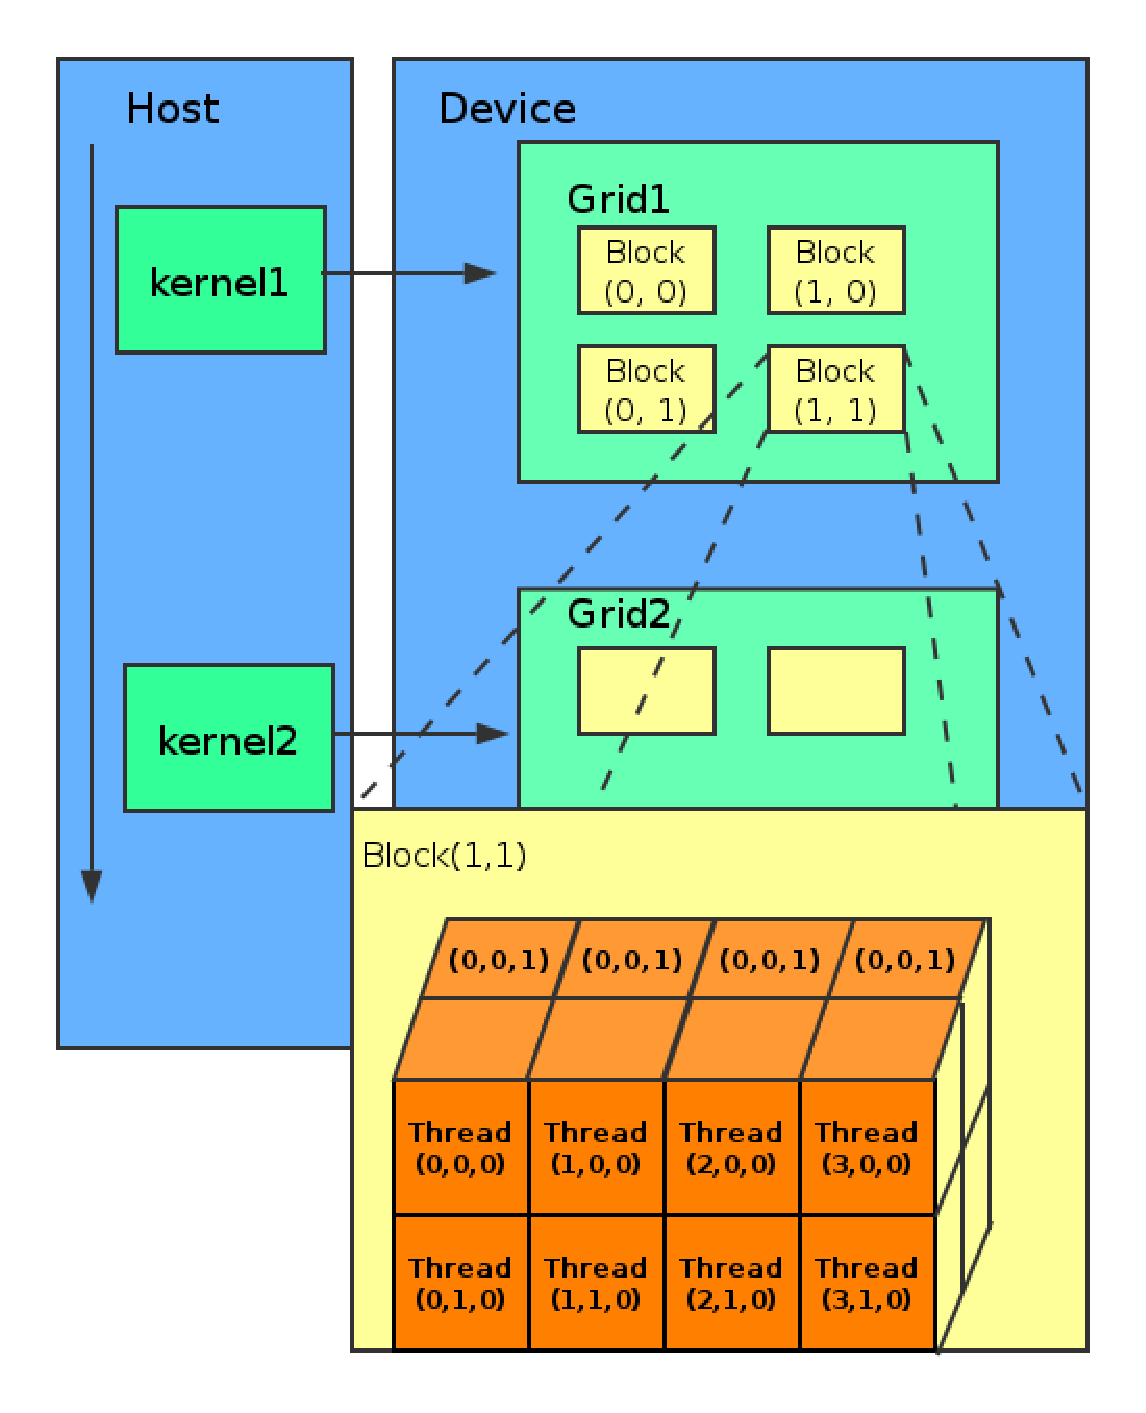
\includegraphics[width=0.6\linewidth]{figure6.eps}
\caption{GPU线程结构}\label{figure6}
\end{figure}
程序运行时,GPU任务分配单元将网格分配到GPU芯片上。CUDA平台启动时,需要将网格配置信息从CPU下发到GPU,
任务分配单元依据配置信息将线程块块分配到多元处理器上。任务分配单元采用轮询策略:轮询遍历多元处理器有没有足够的资源
来执行新的线程块,如果有则给多元处理器分配一个新的线程块。决定是否成功分配的条件有:块运行时需要的寄存器数量,
共享存储器数量,以及其它的一些限制条件。任务分配单元在任务分配中保持公平,然而我们可以通过手动编程设置块内线程数量,
线程使用的寄存器数和共享存储器数来间接控制,保证处理单元负载均衡。任务以这种方法分配使程序具备了很大的可扩展性:
由于每个子任务都能在任意一个多元处理单元上执行,CUDA程序在核心数量不同的处理器上都能正常运行,隐藏了硬件差异。
程序员需要根据具体应用场景将任务拆分为互不相干、可以并行计算的粗粒度子任务,再将每个子任务拆分为能够尽可能利用
线程块内计算资源、存储资源的细粒度指令集。
现有的显卡同一时刻只能执行一个核函数,但是在Fermi架构中可以在同一时刻运行多个核函数。
例如程序员可以在一个内核访问GPU数据的同时,开启另一个内核进行计算,可以很大程度上提高程序运行效率。
线程是串行执行指令的,这就要求每个线程不可以有过多的循环逻辑或者需要过多的存储资源。
当然我们也不应该在单个线程块内分配过多的线程,可能由于参数和中间变量过多导致存储资源不足,降低多元处理器计算速度。
在问题相对复杂时,程序员也可以手动测试一些配置参数的运行速度,选择一个最合适的线程配置参数。

\section{一般代码优化}
程序员编写的代码不总是十全十美,编译器可以自动在不改变程序运行效果的前提下帮助我们进行一些代码优化,使之运行时
的空间效率和时间效率得到提高。编译原理中的代码优化是指通过重排、删除、合并或改变程序片段等策略,使程序代码发生
形式上的改变。本节讨论的是编译阶段的一些代码优化方法,不考虑程序本身算法的效率。
\subsection{变量优化}
任何一个程序离不开变量的定义和变量计算,一些基于变量的简单优化方法可以起到一定的优化效果。表~\ref{table2}给出了
常量合并的传播的优化方法,在编译时就已经可以计算出的常量不需要放到程序执行时计算,减少程序运行时间。
\begin{table}[h]
  \centering
  \caption{常量合并与传播优化}
  \begin{tabular}{p{7cm}<{\centering}p{7cm}<{\centering}}
    \hline
    优化前代码     & 优化后代码   \\
    \hline
    X = 3;         & X = 3;    \\
    Y = X + 2;       & Y = 5; \\
    Z = 3 * Y;      & Z = 15; \\
   \hline
  \end{tabular}
  \label{table2}
\end{table}
表~\ref{table3}描述了公共子表达式外提的优化实例,把两个表达式中重复出现的部分外提出来单独运算,显然优化前
进行了4次加法,优化后进行了3次加法,可以起到一定的加速作用。
\begin{table}[h]
  \centering
  \caption{公共字表达式外提优化}
  \begin{tabular}{p{7cm}<{\centering}p{7cm}<{\centering}}
    \hline
    优化前代码      & 优化后代码   \\
    \hline
    x = b+c+d;      & t = b+c;    \\
    y = b+c+e;      & x = t+d; \\
                    & y = t+e; \\
   \hline
  \end{tabular}
  \label{table3}
\end{table}
还有一些变量优化的场景,比如编译原理中描述的死代码删除。死代码删除是指某个变量的两次定值之间程序没有对该变量的引用,这说明
变量的第一次赋值是多余的,可以删除。一些无用转移语句可以导致一些分支在编译的时候就确定了是否执行,这样编译器可以在编译的时候
就丢弃这些转移逻辑,提升代码执行速度。
\subsection{循环优化}
循环逻辑是程序中重复执行的代码块,对循环结构的优化将会带来更加显著的优化效果。将循环中的不变量或者不变代码外提是最简单的循环优化
方法。表~\ref{table4}中将循环中的不变量2*x+1提出循环外之后,避免了每次迭代时对2*x+1表达式的计算,优化后只需在循环开始之前计算一次,
大大减少了程序运行时间。
\begin{table}[h]
  \centering
  \caption{循环不变量外提}
  \begin{tabular}{p{7cm}<{\centering}p{7cm}<{\centering}}
    \hline
    优化前代码             & 优化后代码   \\
    \hline
    x = c;                    & x = c;    \\
    for(i=0; i<100; i++)      & t = 2*x+1; \\
      array[i] = 2*x+1;       & for(i=0; i<100; i++) \\
	                          &    array[i] = t;  \\
   \hline
  \end{tabular}
  \label{table4}
\end{table}
将循环体内的运算强度削弱也是一种循环优化的方法,在表~\ref{table5}中,我们在循环体内使用加法代替乘法并且得到相同的计算结果。
这种逻辑上的更改不但没有破坏程序结果,而且将每次迭代中的乘法换成了计算强度相对较小的加法,这种优化的效果将随着循环体执行
次数的增加而增加。
\begin{table}[h]
  \centering
  \caption{循环内运算强度削弱}
  \begin{tabular}{p{7cm}<{\centering}p{7cm}<{\centering}}
    \hline
    优化前代码             & 优化后代码   \\
    \hline
    for(i=0; i<100; i++)      & t = 0; \\
       t = i*5;                & for(i=0; i<100; i++)\\ 
                             &    t += 5;\\
  \hline
  \end{tabular}
  \label{table5}
\end{table}











